%
% Niniejszy plik stanowi przykład formatowania pracy magisterskiej na
% Wydziale MIM UW.  Szkielet użytych poleceń można wykorzystywać do
% woli, np. formatujac wlasna prace.
%
% Zawartosc merytoryczna stanowi oryginalnosiagniecie
% naukowosciowe Marcina Wolinskiego.  Wszelkie prawa zastrzeżone.
%
% Copyright (c) 2001 by Marcin Woliński <M.Wolinski@gust.org.pl>
% Poprawki spowodowane zmianami przepisów - Marcin Szczuka, 1.10.2004
% Poprawki spowodowane zmianami przepisow i ujednolicenie 
% - Seweryn Karłowicz, 05.05.2006
% Dodanie wielu autorów i tłumaczenia na angielski - Kuba Pochrybniak, 29.11.2016

% dodaj opcję [licencjacka] dla pracy licencjackiej
% dodaj opcję [en] dla wersji angielskiej (mogą być obie: [licencjacka,en])
\documentclass[magisterska,en]{pracamgr}

% Dane magistranta:
\autor{Joanna Dąbrowska}{438446}

\title{Modeling Genotype to Transcription Interactions in Follicular Lymphoma Using Variational Autoencoder}
\titlepl{Modelowanie zależności między genotypem a transkrypcją w chłoniaku grudkowym z wykorzystaniem wariacyjnego autoenkodera}

% \title{Learning Clonal Architecture of Follicular Lymphoma from Genotype Using a Variational Autoencoder}
% \titlepl{Modelowanie architektury klonalnej chłoniaka grudkowego na podstawie genotypu z wykorzystaniem wariacyjnego autoenkodera}

%kierunek: 
\kierunek{Bioinformatics and Systems Biology}


% Praca wykonana pod kierunkiem:
% (podać tytuł/stopień imię i nazwisko opiekuna
% Instytut
% ew. Wydział ew. Uczelnia (jeżeli nie MIM UW))
\opiekun{dr. Małgorzata Łazęcka\\
  Institute of Informatics\\
  }

% miesiąc i~rok:
\date{September 2024}

%Podać dziedzinę wg klasyfikacji Socrates-Erasmus:
\dziedzina{
11.3 Informatics, Computer Science
}

%Klasyfikacja tematyczna wedlug AMS (matematyka) lub ACM (informatyka)
\klasyfikacja{Applied computing\\
\hspace*{1em} Life and medical sciences\\
\hspace*{2em} Bioinformatics}

% Słowa kluczowe:
\keywords{neural networks, oncology, single cell sequencing, variation autoencoders, VAE}

% Tu jest dobre miejsce na Twoje własne makra i~środowiska:
\newtheorem{defi}{Definicja}[section]
\usepackage{textgreek}
\usepackage{hyperref}
\usepackage{amssymb}
\usepackage{graphicx}
\usepackage{longtable}
\usepackage{booktabs}      % Optional for better horizontal rules
\usepackage[table, dvipsnames]{xcolor} % Optional for coloring
\usepackage{amsmath}
\usepackage{accents}
\usepackage{csquotes}
\usepackage[
backend=biber,
style=nature,
]{biblatex}
\addbibresource{master.bib}
% koniec definicji

\begin{document}
\maketitle

%tu idzie streszczenie na strone poczatkowa
\begin{abstract}
Tumors consist of diverse cell populations exhibiting both genetic and functional heterogeneity, which together influence disease progression and treatment response.
In cancer research, genotype-to-phenotype mapping aims to associate specific genetic alterations in individual cells or clones with functional traits such as transcriptional programs.
Follicular lymphoma, a common non-Hodgkin lymphoma, displays pronounced clonal diversity, yet its genetic and phenotypic heterogeneity have often been studied separately.
A previously developed probabilistic graphical model CaClust integrated multimodal data, including whole-exome, single-cell RNA, and B-cell receptor sequencing, to jointly infer clone genotypes and assign cells to clones, enabling single-cell genotyping.
Building on this foundation, this study proposes a deep learning framework based on variational autoencoders (VAEs) to capture more complex genotype-to-phenotype relationships.
This approach aims to enhance the resolution and interpretability of these links and reveal the functional consequences of somatic evolution in follicular lymphoma.

% Nowotwory składają się z różnorodnych populacji komórek, wykazujących zarówno genetyczną, jak i funkcjonalną heterogeniczność, które wspólnie wpływają na przebieg choroby oraz odpowiedź na leczenie.
% W badaniach nad nowotworami mapowanie genotyp–fenotyp ma na celu powiązanie określonych zmian genetycznych w poszczególnych komórkach lub klonach z cechami funkcjonalnymi, takimi jak programy transkrypcyjne.
% Chłoniak grudkowy, będący jednym z najczęstszych chłoniaków nieziarniczych, cechuje się wyraźną różnorodnością klonalną, jednak jego heterogeniczność genetyczna i fenotypowa były często analizowane oddzielnie.
% Wcześniej opracowany probabilistyczny model graficzny CaClust integrował dane multimodalne, w tym sekwencjonowanie całego egzomu, RNA pojedynczych komórek oraz receptorów komórek B, w celu wspólnego wnioskowania genotypów klonów i przypisywania komórek do odpowiednich klonów, umożliwiając genotypowanie na poziomie pojedynczych komórek.
% W oparciu o tę metodologię, niniejsze badanie proponuje zastosowanie głębokiego uczenia z wykorzystaniem wariacyjnych autoenkoderów (VAE), aby uchwycić bardziej złożone zależności między genotypem a fenotypem.
% Podejście to ma na celu zwiększenie rozdzielczości i interpretowalności tych powiązań oraz ujawnienie funkcjonalnych konsekwencji ewolucji somatycznej w chłoniaku grudkowym.
\end{abstract}+

\tableofcontents

\chapter{Introduction}

\section{General introduction to the topic}

Non-Hodgkin lymphomas are a heterogeneous group of malignancies arising from lymphocytes, and follicular lymphoma (FL) is among the most common indolent forms.
FL is not a single uniform disease but the product of years of subclinical clonal evolution, so a single tumour typically harbours several genetically distinct subpopulations of cells.
Characterising this heterogeneity, meaning which clones are present, how they differ genetically, and how those differences affect cell behaviour, is central to understanding how the disease develops, persists, and sometimes transforms into an aggressive lymphoma.

Single-cell sequencing now makes it possible to measure several molecular layers in the same cell, including its mutation profile, its B-cell receptor sequence, and its gene expression state, in principle allowing a tumour clone's genotype to be related directly to its phenotype.
In practice these measurements are sparse and noisy at single-cell resolution, and combining them into a coherent picture of clonal structure is a non-trivial computational problem.
This work develops and evaluates a computational method for this problem in FL, assigning single cells to their clones and using the result to study how genotype and phenotype are linked.

\section{Biological background}

\subsection{B-cell life cycle}

The B cells are an essential component of adaptive immunity, responsible for producing antibodies. Their development is tightly regulated to generate a highly diverse range of antibodies while ensuring the cells do not attack the body's own tissues.
This developmental progression begins in the bone marrow, where hematopoietic stem cells differentiate into common lymphoid progenitors to seed the B-cell lineage.

Lineage commitment is driven by a network of transcription factors and microenvironmental cues that guide the cells through distinct developmental phases. During the pro-B stage, cells initiate V(D)J recombination to rearrange their immunoglobulin heavy chains.
Upon successful heavy-chain rearrangement, they transition to the pre-B stage to rearrange their light chains.
Once a complete, functional receptor is formed, these newly generated immature B cells leave the bone marrow and migrate to peripheral lymphoid organs, such as the spleen, to complete their maturation.

When these mature B cells encounter an antigen in secondary lymphoid organs, they are triggered to form germinal centers (GCs).
Within these specialized microenvironments, B cells undergo rapid proliferation and activation-induced cytidine deaminase (AID)–dependent modifications, specifically somatic hypermutation (SHM) and class-switch recombination.
Following these genetic modifications, the cells undergo stringent selection; only the clones with the highest affinity for the antigen survive to exit the GC as memory B cells or plasma cells.

Given that GC reactions deliberately introduce DNA breaks and point mutations into immunoglobulin genes to optimize antigen affinity, off-target mutations are an unavoidable byproduct.
Consequently, this AID-mediated mutagenesis is the primary mechanism by which B cells acquire secondary, oncogenic lesions that can initiate or promote lymphoma.
The bone marrow therefore establishes the foundational B-cell repertoire, while the germinal centers are where functional optimization occurs and where the oncogenic mutations that can lead to lymphoma most often arise. \cite{murphy_janeways_2017}

\subsection{Follicular lymphoma}

Follicular lymphoma (FL) is an indolent neoplasm derived from germinal center (GC) B cells, defined by its characteristic nodal architecture of abnormal follicles and by the persistence of a GC-like transcriptional program that circumvents normal selection and exit mechanisms \cite{krull_follicular_2024}. The hallmark initiating lesion in the majority of cases is the t(14;18)(q32;q21) translocation.
This rearrangement places the anti-apoptotic gene BCL2 under the control of the Immunoglobulin Heavy Chain (IGH) locus enhancers.
Since the IGH locus is constitutively and highly active in B cells to support antibody production, its enhancers drive the pathological overexpression of BCL2, providing a profound survival advantage by inhibiting apoptosis.

The presence of t(14;18) alone, however, is not sufficient to establish a precursor state. Small numbers of B cells carrying this rearrangement can be detected in the peripheral blood of a large proportion of healthy adults, reflecting the fact that this event often arises during normal GC reactions. These cells, although genetically altered, do not on their own represent a premalignant stage, and in most individuals they never progress.

A subset of these t(14;18)-bearing cells can evolve into follicular lymphoma–like cells (FLLCs).
These are atypical memory B cells that have transited through the GC and acquired characteristics reminiscent of centrocytes, including CD10+/–, CXCR4$^{\text{low}}$, CD27+, Ki67$^{\text{low}}$, and BCL6 expression, along with molecular footprints of AID activity.
FLLCs display the unusual combination of genomic instability and broad dissemination to lymphoid sites such as lymph nodes and bone marrow, yet they remain biologically inert with respect to malignant progression.
One of their distinguishing features is the preferential retention of surface IgM expression, even when the nonproductive allele has undergone class switching, suggesting selective pressure to maintain IgM-mediated signaling. \cite{carbone_follicular_2019}

By contrast, cancer precursor cells (CPCs) represent a further evolutionary step and are considered true premalignant entities.
CPCs accumulate cooperating mutations in epigenetic regulators, as well as transcriptional factors and immune modulators.
These alterations lock the cells in a GC-like program while progressively eroding normal checkpoints of differentiation and selection.
Unlike FLLCs, CPCs are committed to eventual lymphomagenesis and provide the pool from which clinically overt FL arises.
Importantly, CPCs also function as the genetic reservoir for relapse and transformation.
While early relapses may emerge through linear evolution of the dominant FL clone, late relapses and transformation events typically reflect divergent evolution from a shared CPC ancestor that has branched into genetically distinct sublineages \cite{carbone_follicular_2019}.

\begin{figure}[ht]
    \centering
    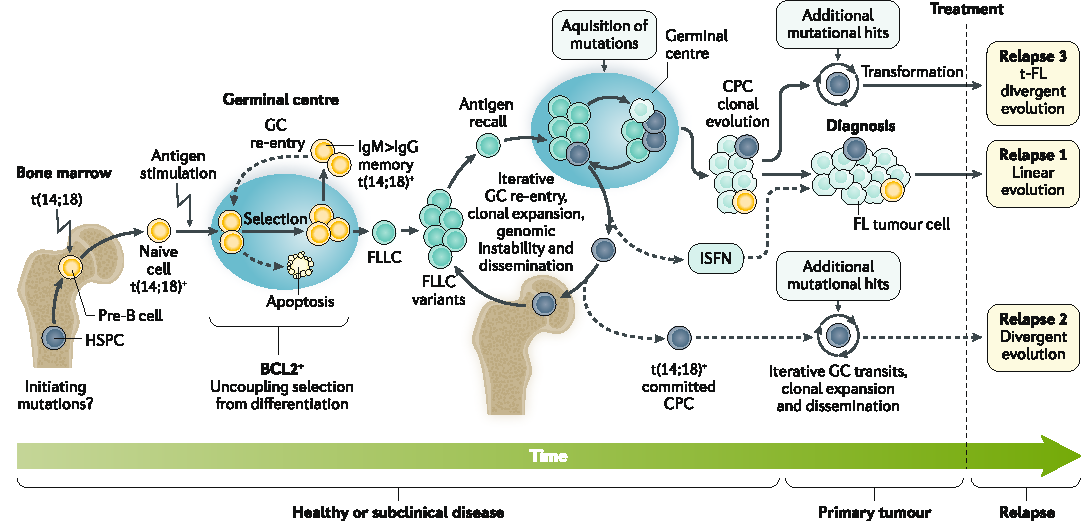
\includegraphics[width=0.9\linewidth]{figures/FL_development.pdf}
    \caption{The stepwise evolution of follicular lymphoma.}
    The development of FL is a long-term process that spans years of subclinical disease. (Left) The process starts with t(14;18) translocations occurring during early B-cell development in the bone marrow or during primary germinal center (GC) reactions. This rearrangement leads to BCL2 overexpression, which prevents apoptosis in cells that would otherwise be eliminated during the normal biological selection process. (Center) These BCL2-expressing cells give rise to follicular lymphoma–like cells (FLLCs) that undergo repeated GC re-entry and spread throughout the lymphoid system. The acquisition of additional mutations, particularly in epigenetic regulators, leads to the emergence of committed cancer precursor cells (CPCs). (Right) CPCs act as a shared ancestral reservoir. While some sublineages evolve directly into the primary tumor found at diagnosis, others remain as a separate pool. This reservoir drives clinical relapse and histological transformation (t-FL) through branched evolution, explaining why relapsed disease is often genetically different from the primary tumor. Figure from \cite{carbone_follicular_2019}
    \label{fig:fl_evolution}
\end{figure}

Once FL is clinically established, the malignant cells remain locked in a GC-like state and persist through iterative GC re-entry, ongoing AID-driven mutagenesis, and selection within the lymphoid niche.
FL primarily involves lymph nodes but frequently extends to the bone marrow and, in some cases, to the peripheral blood.

The tumor microenvironment (TME) is central to sustaining the disease. T$_{\textit{FH}}$ cells provide CD40L, IL-4, and IL-21, which contribute to NF-κB and JAK–STAT pathway activation in tumor B cells \cite{krull_follicular_2024}\cite{carbone_follicular_2019}.
Follicular dendritic and stromal cells produce CXCL12 and CXCL13 that support migration and survival, while macrophages together with regulatory T cells contribute to local immune suppression\cite{carbone_follicular_2019}.

Tumor-intrinsic mechanisms take advantage of these interactions. N-glycosylation of the BCR enables antigen-independent signaling, which drives clonal expansion without the need for antigen recognition and increases the probability of acquiring somatic mutations. Among the most crucial of these are alterations in chromatin regulators such as CREBBP and EZH2, which promote immune evasion by mechanisms including downregulation of MHC expression. Loss of TNFRSF14 further strengthens T$_{\textit{FH}}$–stromal crosstalk, and stromal polarization by neutrophils and macrophages through NF-κB pathways reinforces the supportive niche. \cite{carbone_follicular_2019}

Although usually indolent, FL carries a persistent risk of histologic transformation to an aggressive form, typically diffuse large B-cell lymphoma (DLBCL). Transformation involves the acquisition of aggressive lesions such as TP53 loss, CDKN2A/B deletion, BCL6 rearrangements, or MYC activation, which drive genomic instability, impair cell-cycle checkpoints, and reduce reliance on microenvironmental cues \cite{pasqualucci_genetics_2014}. These genetic and phenotypic changes correspond to the disappearance of follicular architecture, the emergence of diffuse growth, and clinical acceleration with extranodal spread. Whether transformation occurs through a linear accumulation of lesions in the dominant FL clone or through divergent evolution from common precursor cells, both models have been observed, and in either case the outcome is an abrupt shift from indolent to aggressive biology.

\subsection{Current diagnosis and prognostics}

In clinical practice, FL is diagnosed from tissue rather than from molecular data.
The process starts with a biopsied lymph node, which is examined for the abnormal follicular architecture that characterises the disease.
The malignant cells closely resemble normal germinal-center B cells and express the same CD10 and BCL6 markers.
What sets them apart is high expression of BCL2, which normal germinal-center cells do not show \cite{boughan_follicular_2019,alaggio_5th_2022}.

All of these methods read out protein expression and tissue structure rather than the tumour genome.
Sequencing-based molecular testing is therefore not yet a routine part of diagnosis, although liquid-biopsy assays that measure circulating tumour DNA are beginning to add genetic information that tissue examination cannot provide \cite{hamova_circulating_2025}.

Once FL is diagnosed, the clinical question is how aggressively it is likely to behave.
This is answered with prognostic indices computed at diagnosis from routine clinical and laboratory measurements.
The most widely used for risk stratification are the Follicular Lymphoma International Prognostic Index (FLIPI) and its successor FLIPI-2 \cite{mozas_prognostic_2021,jelicic_clinical_2021,jona_prognostication_2025}, which score variables such as patient age, disease stage, haemoglobin level, and measures of tumour burden like the number or size of involved lymph-node areas, and place each patient in a low, intermediate, or high risk group \cite{solal-celigny_follicular_2004,federico_follicular_2009}.

A complementary and more clinically decisive measure is POD24, defined as disease progression within 24 months of starting immunochemotherapy.
Unlike the FLIPI, it is not calculated from baseline variables but observed after treatment, and its value lies in how sharply it separates outcomes.
Patients who progress this early have markedly shorter survival, whereas those who do not have a life expectancy close to that of the general population \cite{casulo_early_2015}.

Purely clinical indices, however, ignore the genetics of the tumour.
The clinicogenetic m7-FLIPI was the first model to close this gap, combining the FLIPI score and performance status with the mutation status of 7 recurrently mutated genes.
The idea behind it is that this molecular information identifies the high-risk, POD24-prone patients more accurately than clinical factors alone \cite{pastore_integration_2015,jurinovic_clinicogenetic_2016}.
Some mutations also carry prognostic weight individually. EZH2 mutations are associated with a more favourable course, whereas TP53 loss and related lesions mark aggressive, transformation-prone disease \cite{jurinovic_clinicogenetic_2016,pasqualucci_genetics_2014}.
Even with these additions, no index can reliably predict the course of an individual patient \cite{boughan_follicular_2019}.

All of these tools, clinical and clinicogenetic alike, work from bulk summaries of the whole tumour.
A different and more basic question is how the genotype of an individual tumour clone relates to the genes its cells express.
That cell level link between genotype and phenotype is the one this thesis sets out to study.

\section{The goal of the study}

Single-cell RNA sequencing (scRNA-seq) measures the transcriptome and does not by itself report a cell's genotype.
Genotype information has to be recovered from reads.
At positions where a somatic mutation is known to occur, the reads covering that position are counted according to whether they carry the reference or the mutant allele.
This produces a second count matrix defined only over the mutated sites rather than over all genes. Because these sites are few and are covered by reads in only a fraction of cells, the matrix is even sparser and more zero-inflated than the already sparse expression matrix, so the genotype signal in any single cell is very weak.

One way to strengthen this signal is to pool information across cells and modalities.
Cells can be grouped by their shared single-nucleotide variant (SNV) profiles, which define clones, and by nearly identical B-cell receptor (BCR) sequences, which define hyperclusters nested within those clones.

This problem has previously been approached with probabilistic graphical models.
CACTUS integrates whole-exome-derived SNV genotypes with scRNA-seq reads at the corresponding loci, pooling the sparse mutation signal across pre-computed cell clusters under the assumption that co-clustered cells share a clone.
CaClust extends this idea by adding the BCR as an explicit modality.
In both models the way the data are generated is specified by hand.
This covers the distribution assumed for each observation, how the underlying clone gives rise to the data and how the two modalities relate to one another.
Because these choices are fixed in advance, the model cannot revise them if the real structure of the data turns out to be different.

This work takes a methodological approach and asks whether a deep generative model, specifically a multimodal variational autoencoder (VAE), is better suited to clone assignment than its probabilistic predecessors.
The VAE still assumes a distribution for each observation, but instead of fixing how the modalities relate to one another and to the underlying clone, it learns these relationships from the data.
The model has two inputs.
The first is the SNV read-count matrix, the same representation used by CACTUS and CaClust.
The second is the BCR sequence of each cell.
Each modality is encoded separately and then mapped into a shared latent space, which is expected to reflect the clonal hierarchy, with BCR hyperclusters forming tight sub-clusters nested inside the broader SNV-defined clones.
Assignment accuracy, together with the quality of the model's genotype reconstructions capabilities, is evaluated against CACTUS and CaClust on FL patient samples and synthetic datasets, which shows how a variational approach performs relative to those models.

Clone assignment is only the first step. Once each cell has been placed in its clone, the gene expression profiles of those cells can be compared across clones to describe how each clone behaves, and these phenotypes can be set against the genetic features that define the clones.
What the model contributes is sharper clonal resolution. By combining the SNV and BCR modalities, it recovers clonal structure that neither modality determines on its own, and this is what makes the downstream comparison possible.
Such comparisons are a starting point for new hypotheses, giving a more detailed view of tumour heterogeneity and clonal evolution and suggesting mechanisms that connect specific genetic lesions to the expression states found alongside them.
\chapter{Materials and methods}

\section{Data}
\subsection{Sample collection and sequencing}
 TO BE PARAPHRASED
 
Samples with histologically confirmed infiltration of follicular lymphoma (FL) grade 1-2 were
collected under authorization of applicable biobank regulations of Leiden University Medical Center and the Ethical Committee of Leiden University Medical Center (reference HEM 008/SH/sh).
Excisional lymph node biopsies were processed immediately by gentle mechanical disruption and mesh filtration.
Single cell suspensions were frozen in 10\% DMSO and remaining tissue fractions were cultured in low-glucose (1g/L) DMEM with 8\% fetal bovine serum to obtain adherent cell cultures for isolation of DNA of cells representing normal counterpart.
Cell processing, library preparation and sequencing FL cells were thawed and purified by flowcytometry using anti-CD19-APC (Becton Dickinson, Franklin Lakes, NJ) and anti-CD10-PECy7 (Becton Dickinson) followed by removal of dead cells (MACS Dead Cell Removal Kit, Miltenyi Biotech, Bergisch Gladbach, Germany).
For whole exome sequencing, DNA was isolated from 1 · 10 6 purified FL cells and from 0.5 · 10 6 cultured adherent cells (Allprep DNA/RNA Mini Kit, Qiagen, Hilden, Germany).
Whole exomes were sequenced using SureSelect Human All Exon V7 baits (Agilent, Santa Clara, CA). Adherent cells representing normal cells were sequenced at 50x coverage.
To discriminate between early clonal variants and more recently acquired subclonal variants as putative drivers of distinct clones, FL bulk DNA was sequenced at 1500x coverage to allow reliable calling of rare variants down to a variant allele frequency (VAF) of 0.02.
For 5’ based single cell transcriptome sequencing, 1 · 105 similarly purified viable cells were loaded on a Chromium X single cell device to generate cDNA libraries for an expected 6 · 103 - 8 · 103 cells per sample. 
The amplified library is split in 3 fractions for 1) full transcriptome sequencing, 2) enrichment of BCR transcripts followed by full length sequencing, 3) targeted resequencing of subclonal somatic variants. Sequencing for WES and single cells was performed on HiSeq2500 or HiSeq4000 devices.

\subsection{Data processing}
 TO BE PARAPHRASED
 
FASTQ files from whole exome sequencing (WES) were processed using the Sarek workflow v2.7
and aligned to the human reference genome GRCh38 using Burrows Wheeler Algorithm (BWA)
v0.7.17. [33, 34] Duplicated mapped reads were marked, local realignment of regions flanking
indels and recalibration of base quality scores were performed to obtain more accurate bases
according to the Genome Analysis ToolKit (GATK) best practices version v4.1.7.0. [35] Sin-
gle nucleotide variants (SNV) and short insertions and deletions (INDELS) were called using
Strelka2 v2.9.10. [36] Only high confidence variants defined by quality scores (GQX) of at least
15 for SNV and 30 for INDELS were kept. Pathogenecity of variants was determined using
the Geneticist Assistant NGS Interpretive Workbench (SoftGenetics) based on publicly avail-
able variant-databases (dbSNP, ClinVar, and COSMIC) and literature, into class 1 (benign),
class 2 (likely benign), class 3 (unknown significance), class 4 (likely pathogenic), or class 5
(pathogenic) [37–39].
20
Variant selection for CaClust modeling
We chose only somatic single nucleotide variants called from Strelka that could also be observed
in the scRNA data of the cells with complete BCR heavy and light chain sequences, and that
showed at least one alternate read across the cells.
Some germline variants were present in the Strelka output, as they had an increased frequency
of the alternate nucleotide over the normal sample. We chose to include only those variants that
showed over 3-fold increase in the frequency of the alternate nucleotide between the normal and
tumour sample. The full table of included variants per sample can be seen in Additional File 3:
Output profiles

\subsection{Generating sample data}
- hyperclusters -> Chinese restaurant process
- hc to clone assignment -> categorical distribution
- bcr sequence -> generate bcr profile using dirichlet distribution for each hypercluster, ans then sample sequence from
categorical distribution across ATGC with probabilities from the profile
- generate raw counts of genes using poisson distribution -> should be NB in fact ;)
- generate clone profiles using binomial distribution
- generate mutation  ounts matrix

\section{Quick introduction to variation auto encoder}
\section{Loss function}
\section{Model description}

\chapter{Results}

\section{Metrics}
\section{Model comparison}
\include{body/discussion}

\cleardoublepage
\addcontentsline{toc}{chapter}{Bibliography}
% \bibliographystyle{abbrv}
% \bibliography{master}
\printbibliography

\cleardoublepage
\addcontentsline{toc}{chapter}{List of figures}
\listoffigures

\cleardoublepage
\addcontentsline{toc}{chapter}{List of tables}
\listoftables

% \appendix
% \include{A_supplementary_graphics}
% \include{B_params_table}
% \include{C_markers_table}

\end{document}
